\clearpage
\section{FIELDS AND FORMS ON MANIFOLDS}
Let $M$ beak-dimensional manifold in $\F{R}^n$ and let $f: W\to \F{R}^n$
be a coordinate system around $x = f(a)$. Since $f'(a)$ has rank $k$, 
the linear transformation $f_*:\F{R}^k_a\to\F{R}^n_x$ is 1-1, and $f_*(\F{R}^k_a)$
is a $k$-dimensional subspace of $\F{R}^n_x$. If $g:V\to\F{R}^n$ is another coordinate
system, with $x=g(b)$, then 
\begin{align*}
    g_*(\F{R}^k_b) = f_*(f^{-1}\circ g)*(\F{R}^k_b) = f_*(\F{R}^k_a)
\end{align*}

Thus the k-dimensional subspace $f_*(\F{R}^k_a)$ does not depend on
the coordinate system $f$. This subspace is denoted $M_x$, and
is called the tangent space of $M$ at $x$ (see Figure \ref{Fig 5-5}).
In later sections we will use the fact that there is a natural inner
product $T_x$ on $M_x$, induced by that on $\F{R}^n_x$: if $v,w\in M_x$ define
$T_x\langle v,w\rangle = \langle v,w\rangle x$.

\begin{figure}[!htb]
    \centering
    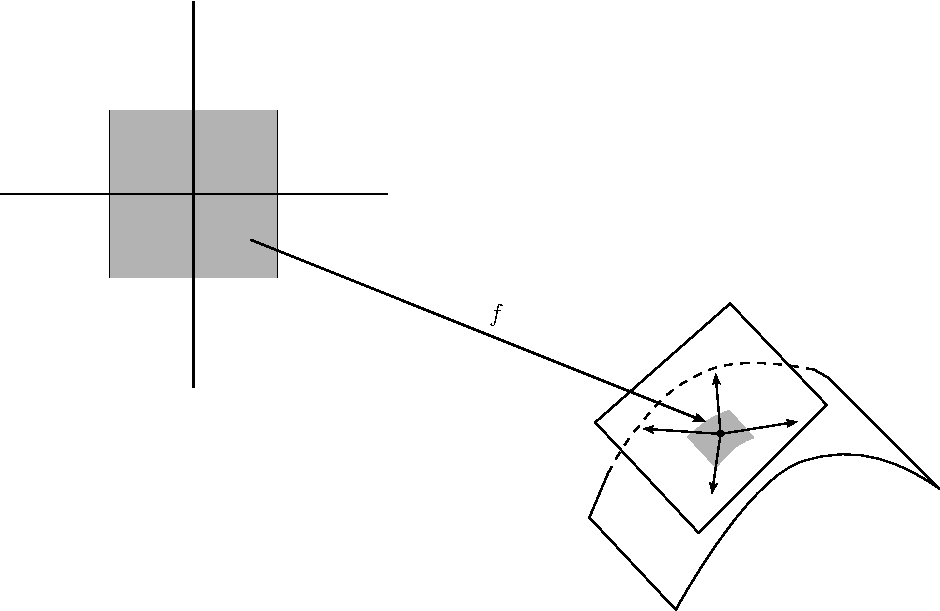
\includegraphics[width=.75\linewidth]{./pics/Fig5-5.pdf}
    \caption{\textit{Some outward unit normal vectors of manifolds-with-boundary in $\F{R}^3$.}}
    \label{Fig 5-5}
\end{figure}

Suppose that $A$ is an open set containing $M$, and $F$ is a differentiable vector 
field on $A$ such that $F(x)\in M_x$ for each $x\in M$. If $f:W\to \F{R}^n$ is a coordinate 
system, there is a unique (differentiable) vector field $G$ on $W$ such that 
$f_*(G(a)) = F(f(a))$ for each $a\in W$. We can also consider a function $F$ which merely assigns 
a vector $F(x)\in M_x$ for each $x\in M$; such a function is called a \textbf{vector field on} $M$. 
There is still a unique vector field $G$ on $W$ such that $f_*(G(a)) = F(f(a))$ for $a\in W$; we 
define $F$ to be differentiable if $G$ is differentiable. Note that our definition does not depend 
on the coordinate system chosen: if $g:V\to\F{R}^n$ and $g_*(H(b))=F(g(b))$ for all $b\in V$, then the 
component functions of $H(b)$ must equal the component fucntions of $G(f^{-1}(g(b)))$, so $H$ is 
differentiable if $G$ is.

Precisely the same considerations hold for forms. A function $\omega$ which 
assigns $\omega(x)\in\Lambda^p(M_x)$ for each $x\in M$ is called a $p-form$ on $M$. If 
$f:W\to \F{R}^n$ is a coordinate system, then $f^*\omega$ is a $p$-form on $W$; we 
define $\omega$ to be differentiable if $f^*\omega$ is. A $p$-form $\omega$ on $M$ can be 
write as 
\begin{align*}
    \omega = \sum_{i_1<\cdots<i_p}^{}{\omega_{i_1,\cdots,i_p}\;\dd x^{i_1}\wedge\cdots\wedge\dd x^{i_p}}    
\end{align*}

Here the function $\omega_{i_1,\cdots,i_p}$ are defined only on $M$. The definition of $\dd \omega$ 
given previously would make no sense here, since $\R{D}_j(\omega_{i_1,\cdots,i_p})$ has no meaning. 
Nevertheless, there is a reasonable way of defining $\dd\omega$.

\begin{theorem}
    There is a unique $(p+1)$-form $\dd\omega$ on $M$ such that for every 
    coordinate system $f:W\to \F{R}^n$ on $M$ and every $a\in W$, we have 
    \begin{align*}
        f^*(\dd\omega) = \dd (f^*\omega)
    \end{align*}
\end{theorem}

\begin{proof}
    If $f:W\to\F{R}^n$ is a coordinate system with $x=f(a)$ and $v_1,\cdots,v_{p+1}\in M_x$,
    there are unique $w_1,\cdots,w_{p+1}$ in $\F{R}^k_a$ such that $f_*(w_i) = v_i$. 
    Define $\dd\omega(x)(v_1,\cdots,v_{p+1}) = \dd(f^*\omega)(a)(w_1,\cdots,w_{p+1})$. One can 
    check that the definition of $\dd\omega(x)$ does not depend on the coordinate system $f$,
    so that $\dd\omega$ is well-defined. Moreover, it is clear that $\dd\omega$ has to be 
    defined this way, so $\dd\omega$ is unique.
\end{proof}

\begin{figure}[!htb]
    \centering
    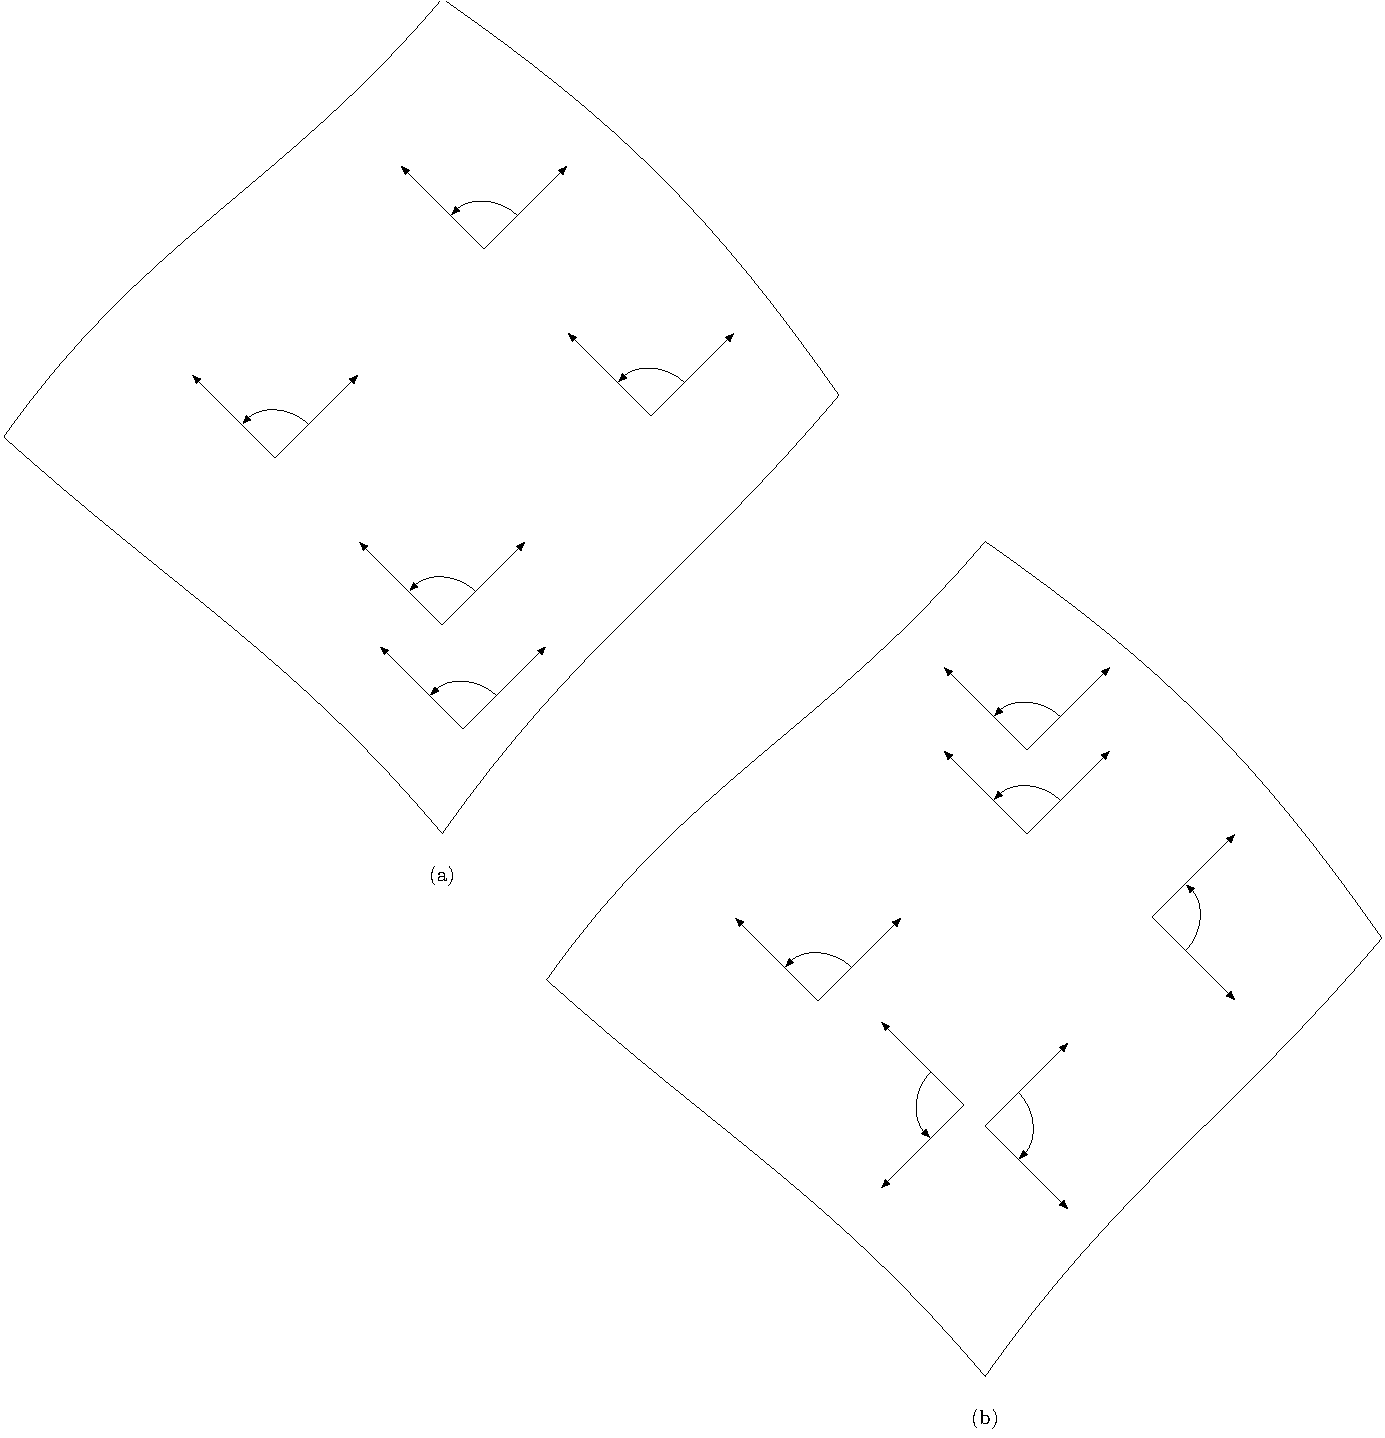
\includegraphics[width=.75\linewidth]{./pics/Fig5-6.pdf}
    \caption{\textit{\textup{(a)} Consistent and \textup{(b)} inconsistent choices of orientations.}}
    \label{Fig 5-6}
\end{figure}

It is often necessary to choose an orientation $\mu_x$ for each
tangent space $M_x$ of a manifold $M$. Such choices are called
\textbf{consistent} (Figure \ref{Fig 5-6}) provided that for every coordinate
$f:W\to\F{R}^n$ and $a,b\in W$ the relation 
\begin{align*}
    [f_*((e_1)_a)], \cdots, f_*((e_k)_a) = \mu_{f(a)}
\end{align*}

holds if and only if 
\begin{align*}
    [f_*((e_1)_b)], \cdots, f_*((e_k)_b) = \mu_{f(b)}
\end{align*}

Suppose orientation $\mu_x$ have been chosen consistently. If 
$f:W\to\F{R}^n$ is a coordinate system such that 
\begin{align*}
    [f_*((e_1)_a)], \cdots, f_*((e_k)_a) = \mu_{f(a)}
\end{align*}

for one, and hence for every $a\in W$, then $f$ is called \textbf{orientation-preserving}.
If $f$ is not orientation-preserving and $T:\F{R}^k\to\F{R}^k$ is a linear transformation with 
$\det T=-1$, then $f\circ T$ is orientation-preserving. Therfore there is an orientation-preserving
coordinate system around each point. If $f$ and $g$ are orientation-preserving and $x=f(a)=g(b)$, then 
the relation 
\begin{align*}
    [f_*((e_1)_a)], \cdots, f_*((e_k)_a) 
    = \mu_x
    = [g_*( (e_1)_b)], \cdots, g_*((e_k)_b)
\end{align*}

implies that 
\begin{align*}
    [(g^{-1}\circ f)_*((e_1)_a), \cdots, (g^{-1}\circ f)_*((e_k)_a)] 
    = [(e_1)_b, \cdots, (e_k)_b]
\end{align*}

so that $\det (g^{-1}\circ f)'>0$, an important fact to remember.

\begin{figure}[!htb]
    \centering
    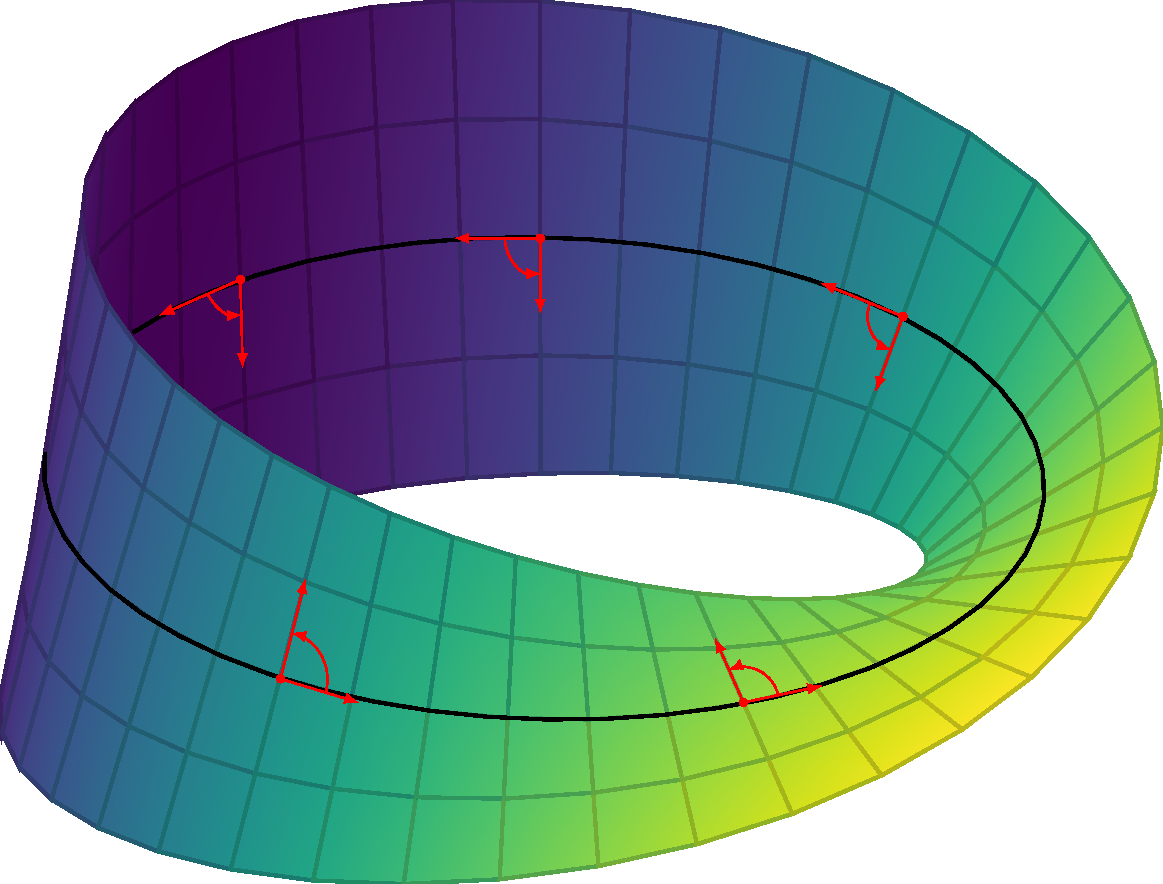
\includegraphics[width=.75\linewidth]{./pics/Fig5-7.pdf}
    \caption{\textit{The M\"obius strip, a non-orientable manifold. A
    basis begins at $P$, moves to the right and around, and comes back to $P$ with
    the wrong orientation.}}
    \label{Fig 5-7}
\end{figure}

A manifold for which orientations $\mu_x$ can be chosen consistently is called \textbf{orientable}, 
and a particular choice of the $\mu_x$ is called an \textbf{orientation} $\mu$ of $M$.
A manifold together with an orientation $\mu$ is called an \textbf{oriented} manifold.
The classical example of a non-orientable manifold is the Mobius strip.
A model can be made by gluing together the ends of a strip of
paper which has been given a half twist (Figure \ref{Fig 5-7}).

Our definitions of vector fields, forms, and orientations can be made for 
manifolds-with-boundary also. If $M$ is a $k$-dimensional manifold-with-boundary 
and $x\in \partial M$, then $(\partial M)_x$ is a $(k-1)$-dimensional subspace of the 
$k$-dimensional vector space $M_x$. Thus there are exactly two unit vectors in $M_x$
which are perpendicular to $(\partial M)_x$; they can be distinguished as follows 
(Figure \ref{Fig 5-8}). If $f: W\to \F{R}^n$ is a coordinate system with $W\subset \F{H}^k$ and 
$f(0) = x$, then only one of these unit vectors is $f_*(v_0)$ for some $v_0$ with $v^k < 0$.
This unit vector is called the \textbf{outward unit normal} $n(x)$; it is not hard to check that this
definition does not depend on the coordinate system $f$.

\begin{figure}[!htb]
    \centering
    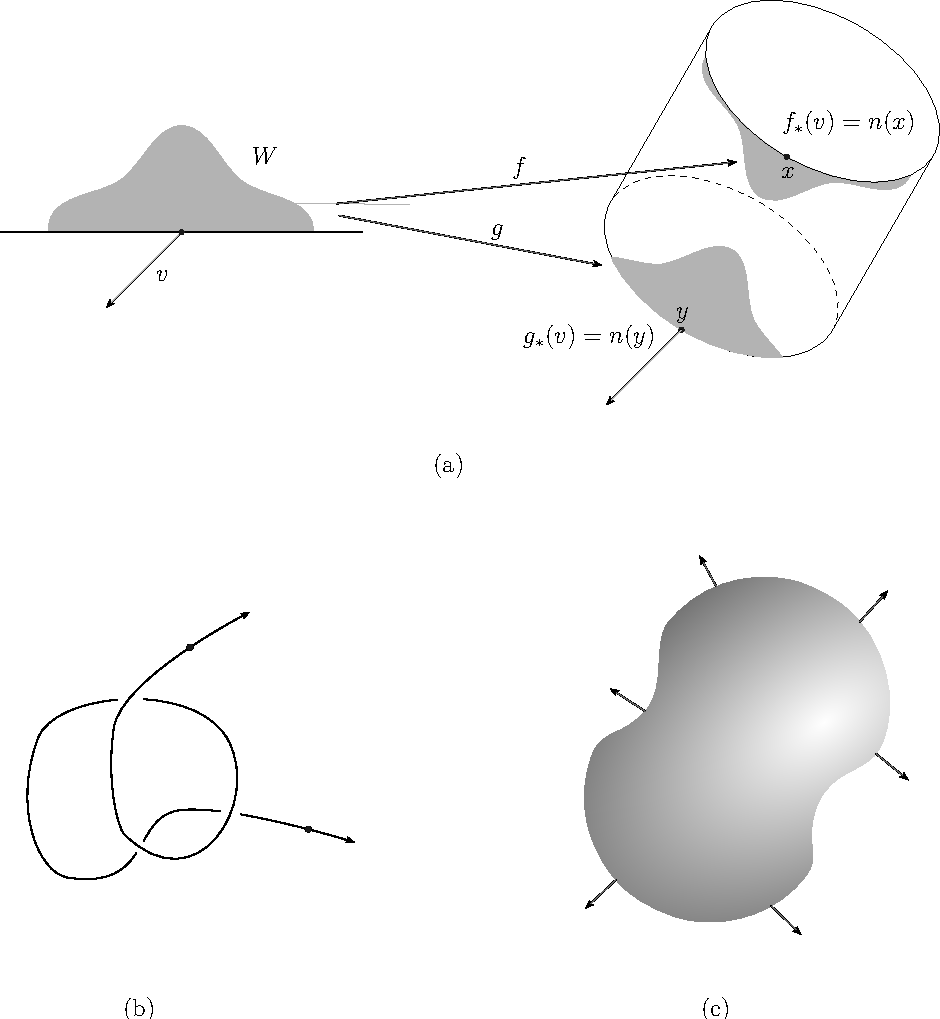
\includegraphics[width=.75\linewidth]{./pics/Fig5-8.pdf}
    \caption{\textit{Some outward unit normal vectors of manifolds-with-boundary in $\F{R}^3$.}}
    \label{Fig 5-8}
\end{figure}

Suppose that $\mu$ is an orientation of a $k$-dimensional manifold-with-boundary $M$. If $x\in\partial M$,
choose $v_1,\cdots,v_{k-1}\in(\partial M)_x$ so that $[n(x), v_1, \cdots, v_{k-1}]=\mu_x$, then both 
$[v_1,\cdots,v_{k-1}]$ and $[w_1,\cdots,w_{k-1}]$ are the same orientation for $(\partial M)_x$. This 
orientation is denoted $(\partial\mu)_x$. It is easy to see that the o  rientation $(\partial\mu)_x$, for 
$x\in\partial M$, are consistent on $\partial M$. Thus if $M$ is orientable, $\partial M$ is also orientable,
and an orientation $\mu$ for $M$ determines an orientation $\partial\mu$ for $\partial M$, called the 
\textbf{induced orientation}. If we apply these definitions to $\F{H}^k$ with the usual orientation, 
we find that the induced orientation on $\F{R}^{k-1}=\{x\in\F{H}^k:x^k=0\}$ is $(-1)^k$ times the usual orientation.
The reason for such a choice will become clear in the next section.

If $M$ is an oriented $(n-1)$-dimensional manifold in $\F{R}^n$, a substitte for outward unit normal 
vectors can be definded, even though $M$ is not necessary the boundary of an $n$-dimensional manifold.
If $[v_1,\cdots,v_{n-1}]=\mu_x$, we choose $n(x)$ in $\F{R}^n_x$ so that $n(x)$ is a unit vector perpendicular 
to $M_x$ and $[n(x), v_1,\cdots,v_{n-1}]$ is the usual orientation of $\F{R}^n_x$. We still call $n(x)$ 
the outward unit normal to $M$ (denoted by $mu$). The vectors $n(x)$ vary continuously on $M$, in an 
obvious sense. Conversely, if a continuous family of unit normal vectors $n(x)$ is defined on all of $M$, 
then we can determine an orientation of $M$. This shows that such a continuous choice of normal vectors is 
impossible pn the M\"obius strip. In the paper model of the M\"obius strip the two side of the paper (which 
has thickness) may be thought of as the end points of the unit normal vectors in both directions.
The impossibility of choosing normal vectors continuously is reflected by the
famous property of the paper model. The paper model is one-sided (if you start to paint it on one 
side you end up painting it all over); in other words, choosing $n(x)$ arbitrarily
at one point, and then by the continuity requirement at other points, eventually forces the 
opposite choice for n(x) at the initial point.


\begin{problems}
    \problem{
        Show that $M$, consists of the tangent vectors at $t$ of curves $c$ in $M$ with $c(t) = x$.
    }
    \problem{
        Suppose $\C{C}$ is a collection of coordinate systems for $M$ such that
        \begin{enumerate}[label=(\arabic*)]
            \item For each $x\in M$ there is $f\in\C{C}$ which is a coordinate system around $x$.
            \item If $f,g\in\C{C}$, then $\det (f^{-1}\circ g)'>0$. Show that there is a unique 
                orientation of $M$ such that $f$ is orientation-preserving if $f\in\C{C}$.
        \end{enumerate}
    }
    \problem{
        If $M$ is an $n$-dimensional manifold-with-boundary in $\F{R}^n$, define
        $\mu_x$ as the usual orientation of $M_x =\F{R}^n_x$, (the orientation $\mu$ so
        defined is the \textbf{usual orientation} of $M$). If $x\in\partial M$, show that
        the two definitions of $n(x)$ given above agree.
    }
    \problem{
        \begin{enumerate}[label=(\alph*)]
            \item If $F$ is a differentiable vector field on $M\subset\F{R}^n$, show that 
                there is an open set $A\supset M$ and a differentiable vector field $\widetilde{F}$
                on $A$ with $\widetilde{F}(x) = F(x)$ for $x\in M$. \textit{Hint:} Do this locally
                and use partitions of unity.
            \item If $M$ is closed, show that we can choose $A=\F{R}^n$.
        \end{enumerate}
    }
    \problem{
        Let $g:A\to\F{R}^p$ be as in Theorem 5-1.
        \begin{enumerate}[label=(\alph*)]
            \item If $x\in M=g^{-1}(0)$, let $h:U\to\F{R}^n$ be the essentially unique diffeomorphism
                such that $g\circ h(y) = (y^{n-p+1},\cdots,y^n)$ and $h(0)=x$. Define that $f_*$
                is 1-1 so that the $n-p$ vectors $f_*((e_1)_0), \cdots, f_*((e_{n-p})_0)$ are linearly
                independent.
            \item Show that orientation $\mu_x$ can be defined consistently, so that $M$ is orientable.
            \item If $p=1$, show that the components of the outward normal at $x$ are some multiple of
                $\R{D}_1g(x), \cdots, \R{D}_ng(x)$.
        \end{enumerate}
    }
    \problem{
        If $M\subset\F{R}^n$ is an orientable $(n-1)$-dimensional manifold, show that 
        there is an open set $A\subset \F{R}^n$ and a differentiable $g:A\to\F{R}^1$
        so that $M=g^{-1}(0)$ and $g'(x)$ has $\R{rank}\;1$ for $x\in M$. \textit{Hint:}
        Problem 5-4 does this locally. Use the orientation to choose consistent
        local solution and use partitions of unity.
    }
    \problem{
        Let $M$ be an $(n-1)$-dimensional manifold in $\F{R}^n$. Let $M(\varepsilon)$ be
        the set of end points of normal vectors (in both directions) of
        length $\varepsilon$ and suppose $\varepsilon$ is small enough so that $M(\varepsilon)$ 
        is also an $(n-1)$-dimensional manifold. Show that $M(\varepsilon)$ is orientable (even if
        $M$ is not). What is $M(\varepsilon)$ if $M$ is the M\"obius strip?
    }
    \problem{
        Let $g:A\to\F{R}^p$ be as in Theorem 5-1. If $f:\F{R}^n\to\F{R}$ is differentiable and the 
        maximum (or minimum) of $f$ on $g^{-1}(0)$ occurs at $a$, show that there are $\lambda_1,\cdots,\lambda_p\in\F{R}$,
        such that
        \begin{align}
            \R{D}_jf(a) = \sum_{i=1}^{p}{\lambda_i\R{D}_jg^i(a)} && j=1,\cdots,n.
            \label{eq:5-2-p16}
        \end{align}

        \textit{Hint:} This equation can be written $\dd f(a)=\sum_{i=1}^{n}{\lambda_i\dd g^i(a)}$ and 
        is obvious if $g(x)=(x^{n-p+1}, \cdots, x^n)$.

        The maximum of $f$ on $g^{-1}(0)$ is sometimes called the maximum of $f$ subject to the 
        \textbf{constraints} $g^i=0$. One can attempt to find $a$ by solving the system of equations \eqref{eq:5-2-p16}.
        In particular, if $g:A\to\F{R}$, we must solve $n+1$ equations
        \begin{align*}
            \R{D}_jf(a) & = \lambda\R{D}_jg(a) \\
            g(a) & = 0
        \end{align*}

        in $n+1$ unknowns $a^1,\cdots,a^n,\lambda$, which is often very simple if we 
        leave the equation $g(a)=0$ for last. This is \textbf{Lagrange's method}, and 
        the useful but irrelevant $\lambda$ is called a \textbf{Lagrangian multiplier}.
        The following problem gives a nice theoretical use for Lagrangian multipliers.
    }
    \problem{
        \begin{enumerate}[label=(\alph*)]
            \item Let $T:\F{R}^n\to\F{R}^n$ be self-adjoint with matrix $A=(a_{ij})$, so 
                that $a_{ij}=a_{ji}$. If $f(x) = \langle Tx, x\rangle = \sum_{}^{}{a_{ij}x^ix^j}$, 
                show that $\R{D}_kf(x) = 2 \sum_{j=1}^{n }{a_{kj}x^j}$. By considering the maximum of 
                $\langle Tx,x\rangle$ on $S^{n-1}$ show that there is $x\in S^{n-1}$ and $\lambda\in\F{R}$
                with $Tx=\lambda x$.
            \item If $V=\{y\in\F{R}^n:\langle x,y\rangle=0\}$ show that $T(V)\subset V$ and 
                $T:V\to V$ is self-adjoint.
            \item Show that $T$ has a basis of eigenvectors.
        \end{enumerate}
    }
\end{problems}